\documentclass[a4paper,10pt]{report}
%\documentclass[a4paper,10pt]{scrartcl}

\usepackage[utf8]{inputenc}
\usepackage{graphicx}
\usepackage{geometry}
\usepackage{wrapfig}
\usepackage{hyperref}
\usepackage{amsmath}
\usepackage{amsfonts}
\usepackage{algorithm}
\usepackage{algpseudocode}
\graphicspath{ {./assets/} }
\hypersetup{
    colorlinks=true,
    linkcolor=blue,
    filecolor=magenta,
    urlcolor=cyan,
    }
\geometry{
 a4paper,
 total={170mm,257mm},
 left=20mm,
 top=20mm,
 }

\title{TIPE simulation de fluide en temps réel}
\author{DERRUAU Noam}
\date{25/10/2023}

\pdfinfo{%
  /Title    (TIPE simulation de fluide en temps réel)
  /Author   (DERRUAU Noam)
}

\begin{document}
\maketitle

\vfill

\begin{abstract}
    Ce document décrit avec précision le travail que je présente dans le cadre de l'épreuve du TIPE 2023/2024 sur le thème 'Jeux et Sports'. Le point de départ de ma réflexion est venu d'une réalisation que l'on observe que très rarement des simulations de fluides interractives dans les jeux vidéos. Certes, dans beaucoup de jeux 'Open World', nous pouvons observer et même nager dans de grandes étendues d'eau, mais celles ci sont toujours statiques, ce sont des animations pré-rendues.\textbf{Le but de ce TIPE est de savoir quelles difficultés interviennent dans la réalisation d'une simulation de fluide newtonien incompréssible en temps réel}.

    Pour ce faire, j'ai codé un moteur de jeu 3D rudimentaire qui a pour seul but de faire le rendu d'une simulation de fluide. J'explique en détail l'architecture du moteur de jeu, la théorie mathématique et physique derrière la simulation de fluide et les différentes approches que l'on peut avoir vis-à-vis de ce problème. Puisque ce travail a pour but de faire parti d'un jeu vidéo, nous négligerons le réalisme au profit des performances. Cependant, le résultat final doit quand même paraître crédible.
\end{abstract}


\newpage
\tableofcontents
\newpage

\chapter{Prérequis}

\section{OpenGL et la programmation graphique}
Pour comprendre le code de ce TIPE, il est nécessaire d'être familier avec OpenGL.
\subsection{Qu'est ce qu'OpenGL?}

OpenGL est une API graphique dont les fonctionnalités sont spécifiés (mais non codés) par le groupe \href{https://www.khronos.org/}{Khronos}. L'implémentation des fonctions est quand à elle laissée aux fabriquants de cartes graphiques (Nvidia, AMD, Intel, etc...). Les librairies graphiques utilisés en interne par notre ordinateur sont donc dépendentes de notre matériel.
Pour mon moteur de jeu, j'utiliserais OpenGL 4.3, version où les {\it compute shaders} ont été introduits.
\\
\begin{wrapfigure}{r}{0.5\textwidth}
    \centering
    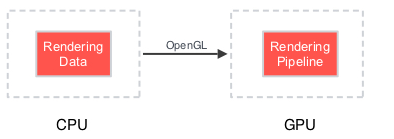
\includegraphics[width=0.5\textwidth]{OpenGL_purpose}
\end{wrapfigure}

Le principe d'OpenGL est d'être une passerelle entre le Processeur et la Carte Graphique, il ne s'occupe pas de la logique de l'application, mais il apporte une couche d'abstraction lors du rendu sur écran.
\\
Pour bien comprendre l'API, il est essentiel d'être au point sur le mode de fonctionnement d'une carte graphique ainsi que certains autres concepts détaillés ci-après.

\subsection{Concepts de base}
\subsubsection{La carte graphique}
Une carte graphique est un composant de l'ordinateur, au même titre que le processeur, dont le but est de transformer des données graphiques envoyés par le processeur en une image cohérente sur un écran. Un processeur est capable d'accomplir cette tache sans l'aide d'une carte graphique, cependant l'opération est très lente et nécessite beaucoup d'optimisation pour tourner avec un nombre d'images par seconde acceptable.

\paragraph{Différence entre un processeur et une carte graphique}
\begin{wrapfigure}{l}{0.5\textwidth}
    \centering
    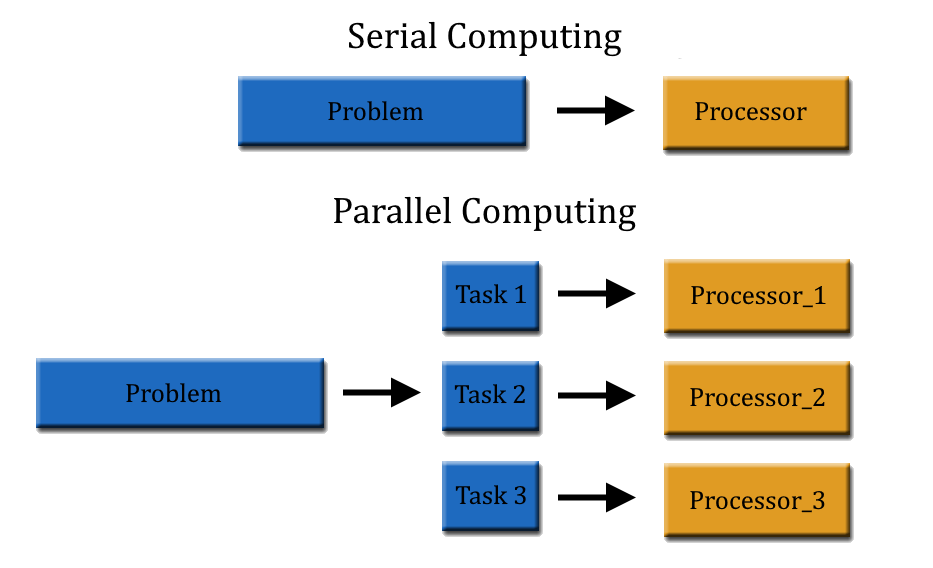
\includegraphics[width=0.5\textwidth]{parallel_computing_vs_sequential_computing}
\end{wrapfigure}
Un processeur moderne va peut être avoir 8 où 16 coeurs qui effectuent autour de 3.5 milliards d'opérations par seconde. Ces coeurs ne sont pas spécialisés, c'est à dire qu'ils peuvent effectuer n'importe quel type de calcul mais ceux-ci sont fait séquentiellement (les uns après les autres).
Une carte graphique moderne va quant à elle avoir autour de 1000 coeurs spécialisés qui effectuent environ 1 millard d'opérations par seconde. Elle excèle lorsque les taches qui lui sont donnés sont faisables en parallèle, c'est à dire que tout les coeurs peuvent travailler sur des petites parties indépendantes et similaires de ladite tache. Le rendu d'image où d'espaces 3D est justement une tache parallélisable, c'est pour cela que le processeur laisse généralement ce travail à la carte graphique

\paragraph{RAM et VRAM}
La mémoire vive (RAM) est un type de mémoire qui permet un accès très rapide aux données, ainsi lorsque vous créez où modifiez une variable dans un programme, celle ci est stockée dans la RAM (on part du principe qu'il n'y a pas de cache) et non sur votre disque dur dont la vitesse d'accès à l'information est 1 million de fois plus lente que sur la RAM. Ainsi rajouter de la RAM vous permettra de stocker plus de données en accès rapide. Cependant, si votre carte graphique a du mal à stocker toutes les données graphiques qu'on lui envoie, rajouter de la RAM ne remédiera pas au problème. Les cartes graphiques possèdes des unités de RAM dédiés et isolés du processeur, appelés VRAM (Video Random Access Memory) directement intégrés à la carte graphique, donc de taille immuable.

\paragraph{Communication entre un processeur et une carte graphique}
La communication entre le processeur et la carte graphique s'effectue au travers d'un cable PCI-Express, qu'on appelle un bus qui possède une grande bande passante. Il n'est pas possible d'accéder directement à une information stockée dans la RAM depuis la carte graphique, ainsi pour afficher un objet 3D à l'écran, il faut d'abord copier cet objet dans la VRAM. De plus, il vaut mieux charger à l'avance dans la VRAM toutes les données que l'on souhaite utiliser, car la communication au travers du bus est très lente. Ce problème est une limitation physique, et donc irrémédiable. En effet, puisque le bus fait aux alentours des $d = 10cm$ de long et que 1 bit d'information traverse le bus à la vitesse de la lumière $c$, on met $t_b = \frac{d}{c}=0.25ns$ pour envoyer un bit. De plus, un seul bit d'information est envoyé par cycle du processeur, donc pour un processeur à $c_s = 4GHz$ qui envoie $i=1Mo$ d'information à la carte graphique, on met $\Delta t = (t_b + \frac{2}{c_s})i = 6.4ms$, ce qui est très lent.

\paragraph{Comment faire un programme qui tourne sur la carte graphique}
Les programmes qui tournent sur la carte graphique sont appelés des shaders. Dans OpenGL, il en existe plusieurs type qui s'exécutent dans cet ordre:
\begin{enumerate}
 \item Le Vertex Shader: il prend en entrée des données quelconques (généralement un point et quelques informations à propos de celui-ci) et retourne une nouvelle position de ce point. À la fin de ce processus le shader forme les \hyperref[subsubsec:Primitives]{primitives} associés à ces points. Les primitives sont les formes de bases associés à des points, par exemple 2 points forment une ligne, 3 points un triangles, etc... On choisit au préalable à quel type de primitives correspondent nos points. Le vertex shader ne mixe pas plusieurs types de primitives.
 \item Le Tesselation Control Shader et Tesselation Evaluation Shader: s'occupe de subdiviser les primitives de base pour lui ajouter des détails tout en interpolants les valeurs supplémentaires associés au point. Les primitives issues de la subdivision sont de même types que la primitive de départ. La subdivision est inscrite dans la primitive de départ, donc cela ne change pas ses contours.
 \item Le Geometry Shader: il prend en entrée une primitive, et permet de retourner une ou plusieurs primitives, dont le type peut être différent.
 \item Le Fragment Shader: Juste après le Geometry Shader se produit l'étape de \href{https://fr.wikipedia.org/wiki/Rast\%C3\%A9risation}{Rastérisation} qui convertit la géométrie en pixels. Après cette étape vient le Fragment Shader. Il permet de définir une couleur pour chacun des pixels issu du Raster. Finalement tout les objets de l'environnement sont placés à leur position respective et l'image finale est créée, c'est l'étape de Color Blending.
 \item Compute Shader: Un programme totalement déconnecté du procédé de rendu graphique, utilisé pour calculer des informations générales de manière parallèle.
\end{enumerate}


\begin{figure}[h]
    \centering
    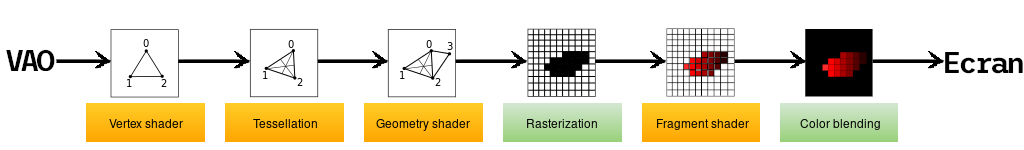
\includegraphics[width=1\textwidth]{shader_pipeline_sideways}
    \caption{Chaine d'éxécution des shaders}
\end{figure}

\paragraph{Les choses à éviter lorsqu'on écrit des shaders} De pars la nature parallèle des shaders, il est déconseillé de faire des programmes qui branchent (if else). En effet, imaginons un programme qui contienne un branchement et que l'une de ses branches mène à un algorithme qui prends beaucoup plus de temps à calculer que celui de l'autre branche. Si sur 100 exécutions du shader, seule une seule valeur prend la branche longue, tout le programme devra attendre que cette branche finisse de s'éxecuter pour renvoyer le résultat final.

\subsubsection{Buffers}
Dans OpenGL, un buffer est une région continue de VRAM qui contient des informations non typés, par exemple cela veut dire qu'on ne dispose d'aucun moyen pour savoir si 01000001 représente le caractère A en ASCII où juste le nombre 65.
Les buffers peuvent soient être mutables soit non-mutables. Ce qu'on veut dire par là, c'est que la taille des buffers et leurs emplacement mémoire n'est pas mutable, mais leur contenu lui l'est. Les buffers non-mutables ouvrent la porte à des optimisations, non détaillés ici.

\subsubsection{Primitives}
\label{subsubsec:Primitives}
Les primitives sont les différents moyens de représenter une suite de points. On peut par exemple dire que la liste $(p_0, ..., p_n)$ représente juste des points de l'espace, mais aussi une suite de segments $[p_ip_{i+1}], \forall i \in  [\![0;n-1]\!]$ ou encore une liste de triangles dont les points $(p_i, p_{i+1}, p_{i+2}), \forall i \in  [\![0;n-2]\!]$ sont les sommets. Dans OpenGL, les primitives disponibles sont les suivantes:

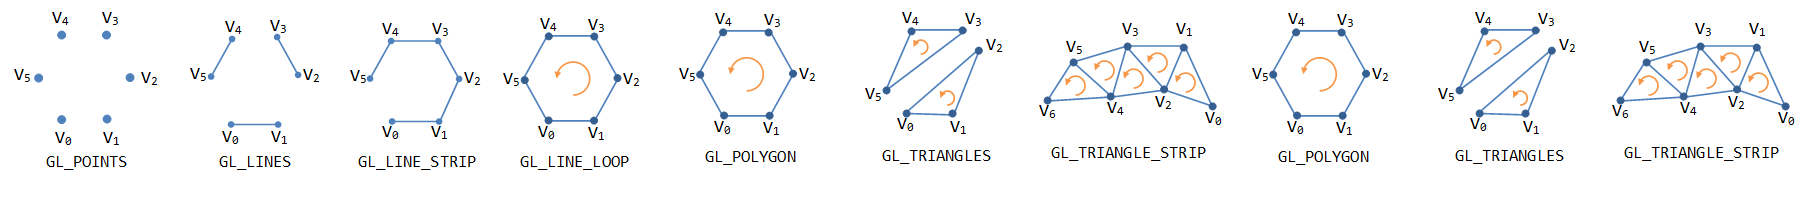
\includegraphics[width=0.96\textwidth]{OpenGL_primitives_flattened}

Notez que les Quads/Polygons ne sont plus disponibles puisque la surface que les points délimitent est ambiguë. En effet, si les 4 points ne sont pas dans le même plan, quels points font partie de la surface?

\subsubsection{Textures}
[WORK IN PROGRESS]

\subsection{Fonctionnement interne d'OpenGL}
[WORK IN PROGRESS]

\subsection{Plus de renseignements}
Ce manuel n'est pas une documentation de la spécification OpenGL 4.3, aussi je ne détaillerais pas plus son fonctionnement. Pour approfondir vos connaissances, je conseille de lire les wikis suivants:
\begin{itemize}
 \item \href{https://www.khronos.org/opengl/wiki/}{Le wiki OpenGL de Khronos}: il permet de comprendre les concepts spécifiques à la libraire et les différents systèmes interagissent entre eux.
 \item \href{http://www.hyzgame.org.cn/OpenGL/man3/bottom.php}{La référence des fonctions OpenGL 3.3}: Contient une liste exhaustive de toutes les fonctions d'OpenGL 3.3 ainsi que comment les utiliser.
 \item \href{https://learnopengl.com}{LearnOpenGL.com}: Un site qui permet d'apprendre les concepts de rendu d'espace 3D avec OpenGL. Il est conseillé d'avoir lu le Wiki de Khronos avant de lire le contenu de ce site
 \item \href{https://www.youtube.com/playlist?list=PLn3eTxaOtL2PDnEVNwOgZFm5xYPr4dUoR}{OpenGL avec Python}: une série de vidéos qui explique comment utiliser OpenGL sous python (utile dans le cadre de ce projet)
\end{itemize}


\chapter{La théorie mathématique et physique}
Dans tout ce chapitre, on se place en coordonnées cartésiennes.
\section{Introduction à la mécanique des fluides}
\subsection{Notion de particule de fluide et configuration d'un fluide}
Une particule de fluide est un volume élémentaire $dV$ centré sur un point $M$ et de masse volumique $\rho$. Les dimensions du volume sont à \href{https://fr.wikipedia.org/wiki/Mésoscopique}{l'échelle mésoscopique}, c'est à dire que ce volume est assez petit pour pouvoir faire du calcul différentiel avec mais assez grand pour étudier le comportement moyen des propriétés des atomes contenus dans ce volume.
À l'instant $t$, une particule de fluide est repérée par l'emplacement $M$ de son centre.

Un fluide est donc défini comme un ensemble de particules de fluide occupant un volume $V$ de l'espace à l'instant $t$. Pour décrire les différentes grandeurs physiques qui caractérisent chaque particule de fluide, on utilisera la notion de champ : champ de vitesse, champ d'accélération, champ de masse volumique, champ de température, de pression, etc... Ces champs caractérisent la grandeur correspondante pour tout point du système étudié.

\subsection{Les différents points de vue}
Il existe 2 grandes écoles de pensée, ceux qui décrivent un fluide de manière Eulerienne et ceux qui décrivent un fluide de manière Lagrangienne. Prenons l'exemple d'une course de Formule 1. On peut assimiler un fluide à un ensemble de voitures qui se suivent, une seule voiture constituant une particule fluide. La configuration initiale serait la situation au départ de la course ; la configuration actuelle serait la situation à un instant donné de la course.

Il faut décrire toute la course, i.e décrire le mouvement de toutes les voitures. Pour cela, deux solutions sont possibles. Soit on met une caméra sur chaque voiture (approche lagrangienne), soit on pose des caméras régulièrement le long de la piste (approche eulérienne). Si on a besoin d’identifier la voiture, dans le premier cas, on sait que la caméra x est sur la voiture qui est partie en xième position (mouvement rigide, approche lagrangienne). Dans le deuxième cas, il suffit de chercher devant quelle caméra passe la voiture (mouvement fluide, approche eulérienne).

\subsubsection{Description Lagrangienne}
Dans le cadre de la \href{https://fr.wikipedia.org/wiki/Description_lagrangienne}{description lagrangienne}, on suit une particule fluide dans son mouvement et on regarde sa position à un instant $t$, notée $M(t)$. Les inconnues de la description de lagrange sont les coordonnées $x$, $y$ et $z$ à l'instant $t$ d'une particule de fluide.
$$\vec{OM}(t) = x(t)\vec{u_x} + y(t)\vec{u_y} + z(t)\vec{u_z}$$
Pour avoir la vitesse et l'accélération, il suffit donc de dériver l'expression de $\vec{OM}$.

\subsubsection{Description Eulerienne}
Dans le cadre de la \href{https://fr.wikipedia.org/wiki/Description_eulérienne}{description eulerienne}, on considère un volume $d\tau$ fixe dans l'espace et on mesure la vitesse (ou une autre propriété) moyenne du fluide pour toutes les particules qui traversent cette région. L'inconnue de la description de euler est donc la vitesse $u(t)$ moyenne des particules de fluide dans ce volume.
$$\vec{u}(t) = u_x(t)\vec{u_x} + u_y(t)\vec{u_y} + u_z(t)\vec{u_z}$$
Pour avoir la position, on intègre cette expression, et pour avoir l'accélération on la dérive.
On arrive à $\vec{a} = \frac{\partial \vec{u}}{\partial t} + \frac{\partial \vec{u}}{\partial x}\frac{\partial \vec{x}}{\partial t} + \frac{\partial \vec{u}}{\partial y}\frac{\partial \vec{y}}{\partial t} +\frac{\partial \vec{u}}{\partial z}\frac{\partial \vec{z}}{\partial t} = \boxed{ \frac{\partial \vec{u}}{\partial t} + \vec{\nabla}\vec{u}\cdot \vec{u} = \vec{a}}$
\begin{center}
 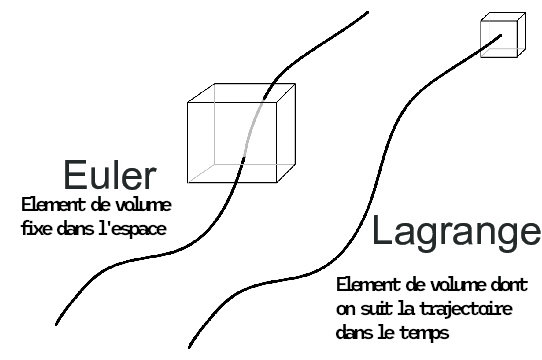
\includegraphics[width=0.5\textwidth]{eulerian_vs_lagrangian_description}
\end{center}

Au final dans les deux cas, on a bien définit le champs de position des particules, cependant avec Euler on doit traquer les particules qui rentrent/sortent de chacun des volumes et avec Lagrange on doit traquer la position des particules en elles même. Pour un programme informatique, la description Lagrangienne est à privilégier, mais pour l'étude théorique, on privilégie la description Eulerienne. Les deux nous mènent aux mêmes résultats.

\section{Les equations de Navier-Stokes}
Maintenant que nous comprenons un peu mieux les fluides, il est temps d'établir l'équation de leur mouvement. Pour cela, considérons une particule de fluide de position $M$ et de masse $m$ à laquelle on veut appliquer la 2eme loi de Newton. On distingue deux types de forces appliqués à cette particule:
\begin{itemize}
 \item Les forces de contact: les forces entre deux particules de fluides qui se touchent.
 \item Les forces à distance: les forces issues du poids $\vec{P}$, de la force de Lorentz, etc...
\end{itemize}

La 2nde loi de newton s'écrit donc:
\begin{align*}
m \frac{d\vec{v}}{dt} &= \vec{F}_{contact} + \vec{F}_{distance}
\end{align*}
 On remarque que les forces à distances sont généralement définies volumiquement, c'est à dire que l'on peut factoriser un élément $d\tau$ à la force. Par exemple, le poids:
 $$\vec{P} = m\vec{g} = \rho d\tau \vec{g}$$
 On aimerait donc bien sortir un $d\tau$ de chacunes des forces pour pouvoir le simplifier dans la 2nde loi de Newton. Pour cela, il nous faut trouver un équivalent volumique de chacune d'entre elles.

 \subsection{Les forces de contact}

\begin{wrapfigure}{r}{0.4\textwidth}
 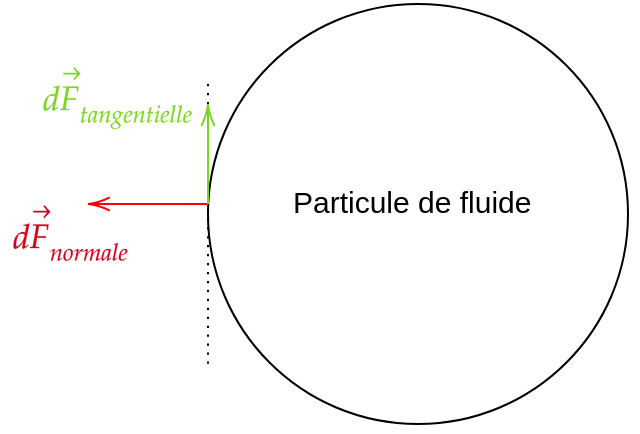
\includegraphics[width=0.4\textwidth]{force_de_contact_particule_de_fluide}
\end{wrapfigure}
Pour un élément de surface $\vec{dS}$ de la particule de fluide, on peut définir une force infinitésimale de contact $d\vec{F}_{contact}$ décomposable comme ceci:
$$d\vec{F}_{contact} = d\vec{F}_{tangentielle} + d\vec{F}_{normale}$$
On nomme la composante tangentielle de la force de contact la \textbf{viscosité} et la composante normale la \textbf{pression}. Par convention, la composante normale est orientée sortant de la particule de fluide.
% Pour éviter les collisions entre les 2 wrapfigure
\\
\\
\\
\newpage

\subsubsection{Equivalent volumique de la force de pression}
\begin{wrapfigure}{r}{0.2\textwidth}
 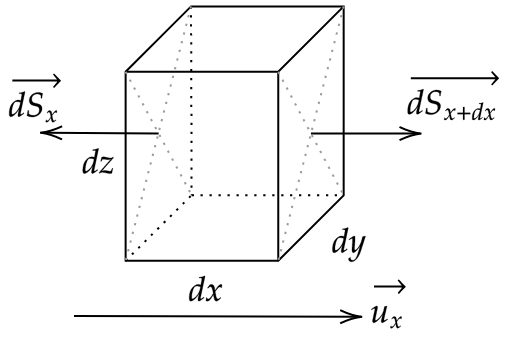
\includegraphics[width=0.2\textwidth]{equivalent_force_de_pression_volumique}
\end{wrapfigure}
On considère un élément de volume $d\tau = dxdydz$. On note $P$ le champs de pression définit dans l'espace. La force de pression $dF_x$ exercée sur l'élément $d\tau$ sur l'axe $\vec{u_x}$ est définie de cette façon:
\begin{align*}
 dF_x &= P(x,y,z)dydz - P(x+dx, y, z)dydz \\
           &= - (P(x+dx, y, z) - P(x, y, z))dydz \\
           &= - \frac{\partial P}{\partial x} dxdydz \\
           &= - \frac{\partial P}{\partial x} d\tau
\end{align*}
 En généralisant à 3 dimensions on obtient:
$$ \boxed{\frac{\vec{dF_{pression}}}{d\tau} = - \vec{\text{grad}}P} $$
\\
\subsubsection{Equivalent volumique de la viscosité}

\begin{wrapfigure}{l}{0.4\textwidth}
 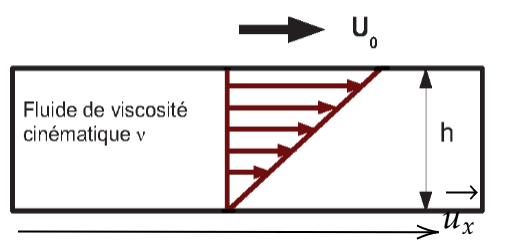
\includegraphics[width=0.4\textwidth]{ecoulement_couette_plan}
  \caption{\href{https://fr.wikipedia.org/wiki/écoulement_de_Couette}{Écoulement couette plan}}
\end{wrapfigure}
Dans cette situation, on considère une lame de fluide de hauteur $h$. La couche du haut est une plaque solide qu'un opérateur tire à la vitesse $\vec{u_0}$. On remarque que pour chaque couche de fluide, la couche d'au dessus l'entraine et la couche du dessus la freine, ce qui crée une vitesse qui diminue linéairement avec la distance à la plaque. On a l'expression de la vitesse:
$$ \vec{v} = v_x(y)\vec{u_x}$$
Par aileurs: on définit la force de viscosité volumique par:
$$ \vert \vec{V}dS \vert =\vert \frac{d \vec{F_{viscosite}}}{d S} \vert = \eta \vert \frac{\partial \vec{v}}{dy} \vert$$

\begin{wrapfigure}{r}{0.2\textwidth}
 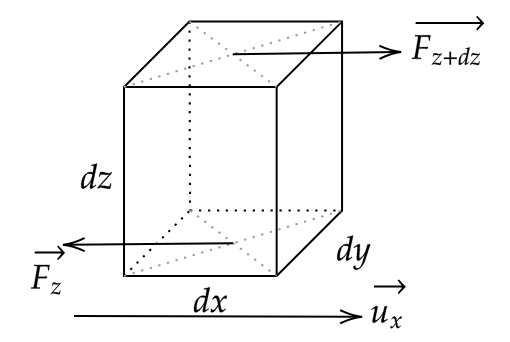
\includegraphics[width=0.2\textwidth]{equivalent_force_de_viscosite_volumique}

% 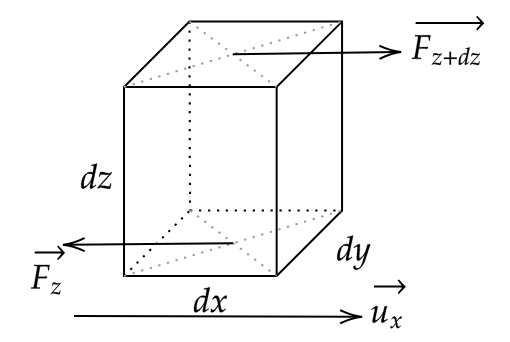
\includegraphics[width=0.2\textwidth]{equivalent_force_de_viscosite_volumique}
\end{wrapfigure}
On peut donc faire le bilan de la force de viscosité $dF_x$ sur l'axe $u_x$ sur un petit élément $d\tau = dxdydz$
\begin{align*}
 dF_x &= \eta \frac{\partial v_x}{\partial y}(x, y, z + dz) dxdy - \eta \frac{\partial v_x}{\partial y}(x, y, z) dxdy \\
      &= \eta (\frac{\partial v_x}{\partial y}(x, y, z + dz) - \frac{\partial v_x}{\partial y}(x, y, z)) dxdy \\
      &= \eta \frac{\partial^2 v_x}{\partial y^2} ddydxdz \\
      &= \eta \frac{\partial^2 v_x}{\partial y^2} d\tau
\end{align*}
\\
En généralisant à 3 dimensions, on obtient:
$$ \boxed{\frac{d\vec{F_{viscosite}}}{d\tau} = \eta \Delta \vec{v} }$$

\newpage
\subsection{Établissement de l'équation de Navier-Stokes}
Maintenant que nous avons nos forces volumiques, il suffit de les mettre dans la 2nde loi de Newton:
$$ \boxed{\rho \frac{d\vec{v}}{dt} = \rho \vec{g} - \vec{grad} P + \eta \Delta \vec{u} + \vec{F}}$$

où $\vec{F}$ sont toutes les forces supplémentaires en dehors des actions de contact et du poids ($\rho \vec{g}$).
Cette équation est valable pour un fluide incompréssible, c'est à dire un fluide où $\frac{d \rho}{dt} = 0$

\subsubsection{Compléments à l'équation de Navier-Stokes - Equation de continuité}
Une seconde équation peut être formulée pour les équations de Navier-Stokes. Celle ci vient du fait qu'un fluide obéit à la conservation de la masse. C'est à dire que le fluide ne peut spontanément être créé depuis une source ou spontanément détruit par un puit.
\begin{center}
 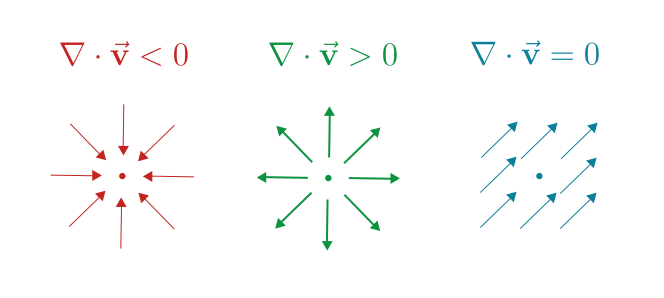
\includegraphics[width=0.8\textwidth]{equation_de_continuite_navier-stokes}
\end{center}
On arrive après quelques calculs à l'équation:
$$ \frac{d \rho}{dt} + \rho \text{div } \vec{v} = 0$$
Ce qui donne dans le cas d'un fluide incompréssible:
$$ \boxed{\text{div } \vec{v} = 0} $$

\vfill
Pour résumer, les équations de Navier-Stokes sont:
$$
\boxed{\begin{cases}
 \text{div } \vec{v} = 0 & \text{Equation de continuité où de conservation de la masse} \\
 \rho (\frac{\partial \vec{u}}{\partial t} + \vec{\nabla}\vec{u}\cdot \vec{u} ) = \rho \vec{g} - \vec{grad} P + \eta \Delta \vec{u} + \vec{F} & \text{Equation de conservation de la quantité de mouvement}
\end{cases}}
$$
\vfill
\newpage

\section{L'algorithme SPH}

\subsection{Principe de l'algorithme}
L'algorithme SPH, acronyme de '\href{https://en.wikipedia.org/wiki/Smoothed-particle_hydrodynamics}{Smoothed Particle Hydrodynamics}' vise à résoudre les équations de Navier-Stokes en considérant le fluide comme un ensemble discret de particules de fluide, chacune de rayon $r$ et de masse $m$. Ce point de vue offre de nombreux avantages puisque le nombre constant de particules de masse constante dans la simulation garantie le respect de l'équation de conservation de la masse.

De plus, on peut rempalcer le terme $\frac{\partial \vec{u}}{\partial t} + \vec{\nabla}\vec{u}\cdot \vec{u}$ par $\frac{d \vec{u}}{dt}$. En effet, le terme $\frac{\vec{u}}{\partial t} + \vec{\nabla}\vec{u}\cdot \vec{u}$ est appelé le terme \href{https://fr.wikipedia.org/wiki/Advection}{d'advection}. C'est à dire qu'il correspond à la variation de la vitesse de la particule dûe au déplacement du fluide. Or comme les particules \textbf{sont} le fluide, ce terme est nul (je suis pas sûr de ma justification mais je crois les mots de \textit{Muller}). On se retrouve à devoir trouver des approximations discrètes des termes $\rho \vec{g}$, $\vec{grad} P$, $\eta \Delta \vec{u}$ et $\vec{F}$.

Pour finir, comme les équations de Navier-Stokes sont générales pour les fluides, elles n'incluent pas la tension de surface. Nous devrons donc la modéliser et la représenter séparément.
\subsection{Prérequis}
\subsubsection{La pseudo-fonction de Dirac}
La pseudo-fonction de Dirac est un objet mathématique qui possède ces propriétés:
\begin{align*}
 \delta(x) =
\begin{cases}
  + \infty & \text{si } x=0 \\
  0 & \text{sinon}
 \end{cases} \\
 \int_{-\infty}^{+\infty} \delta(x)dx = 1
\end{align*}

Ce n'est pas une fonction mathématique usuelle, mais une \href{https://fr.wikipedia.org/wiki/Théorie_de_la_mesure}{mesure}.

On définit usuellement cette pseudo-fonction comme limite d'une suite de fonctions. Par exemple soit
$
f_n(x) =
\begin{cases}
 n & \text{si } x\in [\frac{-1}{2n}, \frac{1}{2n}] \\
 0 & \text{sinon}
\end{cases}
$
une suite de fonction CM et intégrable sur $\mathbb{R}$. On a bien $f_n \underset{s}{\to} \delta$ et
\begin{align*}
 \lim_{n\to +\infty} \int_{-\infty}^{+ \infty} f_n(x)dx &=\lim_{n\to +\infty} \int_{-\frac{1}{2n}}^{\frac{1}{2n}} ndx & \text{Changement de variable } u=2nx\\
 &= \lim_{n\to +\infty} \int_{-1}^{1} \frac{1}{2}dx & \text{integration sur un segment: on peut rentrer la limite dans l'intégrale}\\
 &= 1 &
\end{align*}
$\delta$ est bien limite de cette suite de fonctions.
\\
De plus, soit $g$ une fonction continue et intégrable sur $\mathbb{R}$.

\begin{align*}
 \int_\mathbb{R} g(x)\delta(x-t)dx &= \lim_{n \to +\infty} \int_{-\frac{1}{2n}}^{\frac{1}{2n}} g(x) n dx & \text{changement de variable } u=2n(x-t) \\
 &= \lim_{n \to + \infty} \int_{-1}^1 g(t + \frac{u}{2n})\frac{1}{2}du \\
 &= g(t)\int_{-1}^1 \frac{1}{2}du \\
 &= g(t)
\end{align*}

On peut donc écrire cette identité pour le Dirac:
$$\boxed{ \int_\mathbb{R} g(x)\delta(x-t)dx = g(t)}$$
\newpage
\subsubsection{Noyau de lissage}
En statistique, pour extrapoler une fonction continue et lisse $\hat{f}_h$ (au sens des variations) à partir d'un échantillonnage de $n$ points $X_1, ... X_n$, on utilise la technique \href{https://fr.wikipedia.org/wiki/Estimation_par_noyau}{d'estimation par noyau}. On estime que:
$$\hat{f}_h(x) = \frac{1}{nh} \sum_{i=1}^n K(\frac{x - x_i}{h})$$
où
\begin{itemize}
 \item $h$ est le paramètre de lissage: plus il est grand, plus la fonction est lissée
 \item $K$ est une fonction noyau de lissage. Elle assigne un 'poids de contribution' au point $x_i$ pour la valeur de la fonction $\hat{f}_h$ au point $x$ d'autant plus fort que $\frac{x - x_i}{h}$ est proche de 0. De plus $\underset{x\to \pm \infty}{\lim} K(x) = 0$
\end{itemize}

Pour être plus précis, on estime que la valeur d'une fonction en un point $x$ est environ égal à la moyenne des positions des points $X_i$ qui sont proches de $x$, ceux étant éloignés sont négligeables donc leur poids par la fonction $K$ est approximable à 0.
\begin{figure}[h]
\begin{center}
 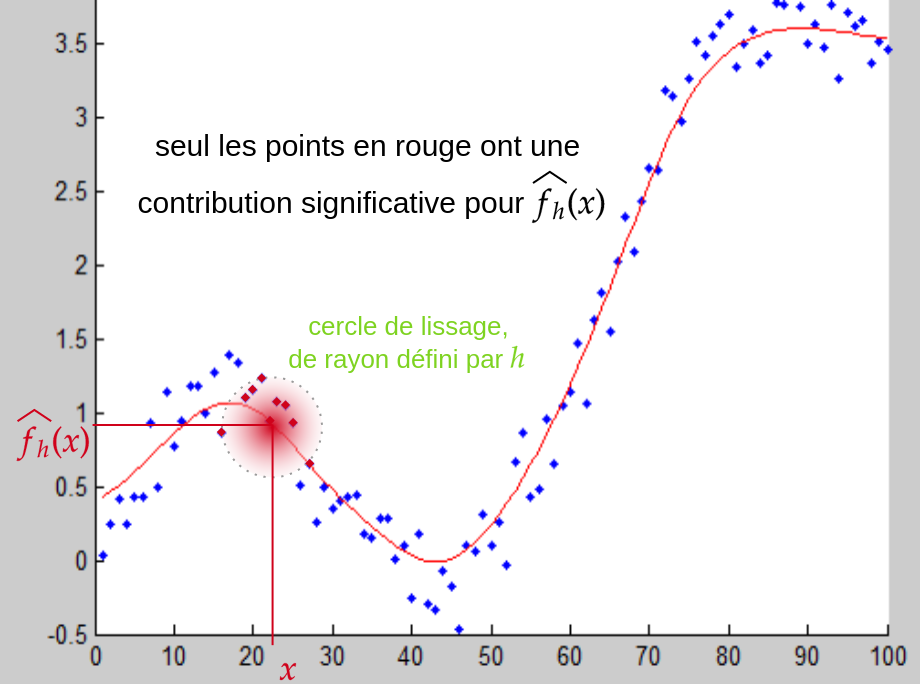
\includegraphics[width=0.8\textwidth]{kernel_smoother_graph}
\end{center}
 \caption{Explication intuitive de la fonction lissée}
\end{figure}

On pose $r= \lVert X - X_i \rVert$ la distance entre le point étudié $X$ et un point $X_i$.

Les fonctions de lissage $K$ sont de la forme $K(r, h) = \frac{\sigma}{h^d}f(\frac{r}{h})$ où $d$ est le nombre de dimensions sur lequel on travail (3 dans notre cas) et $\sigma$ est un coefficient de normalisation. On pose $\mathbf{q = r/h}$. La fonction $K$ doit répondre à certains critères:
\begin{align*}
 & K \text{ positive, définie et décroissante} \\
 & \lim_{h \to 0}K(r,h) = \delta(r) \\
 & \sigma \int_\mathbb{R} f(q)dV = 1 & \text{où } dV = 4\pi q^2 dq \text{ en dimension 3}
\end{align*}

La première fonction à laquelle nous pouvons penser comme candidat de noyau de lissage est la fonction Gaussienne:
$$K(r,h) = \frac{1}{\pi\sqrt{\pi} h^3}e^{-(r/h)^2}$$
Cependant, nous n'utiliserons pas cette fonction à cause de son cout en temps pour un ordinateur . Il est préférable d'utiliser des polynomes plus rapides à calculer. De plus la fonction gaussienne n'est pas à support compact (i.e $\text{supp}(f) = \overline{\{x \in \mathbb{R}, f(x) \neq 0 \}}$ n'est pas un compact). C'est génant car lors de l'analyse mathématique, nous ne pouvons plus négliger les points loin en distance. Je propose donc d'utiliser la fonction suivante, où $\mathbf{q = r/h}$
$$\boxed{
K(r,h) = \frac{1}{\pi h^3}
\begin{cases}
 1 - \frac{3}{2}q^2 + \frac{3}{4}q^3 & \text{si } 0 \le q < 1 \\
 \frac{1}{4}(2-q)^3 & \text{si } 1 \le q < 2 \\
 0 & \text{si } q \ge 2
\end{cases}}$$
C'est un polynome à support compact de taille $2h$.

\subsection{Approximation discrète de champs scalaire et de champs vectoriels}
L'objectif de cette partie est d'obtenir l'approximation d'un champs scalaire/vectoriel continu sur l'espace en s'inspirant de la technique d'estimation par noyau.

\subsubsection{Approximation pour un champs scalaire}
Soit $A: \mathbb{R}^3 \to \mathbb{R}$ un champs scalaire.

On part de l'identité du Dirac: $$A(M) = \int_{\mathbb{R}^3} A(M')\delta(\lVert M' - M\rVert)d^3M'$$.
On pose similairement \\$$<A>(M) = \int_{\mathbb{R}^3} A(M')K(\lVert M' - M\rVert, h)d^3M'$$ où $K$ est une fonction lissage de noyau.
On cherche à connaitre l'ordre de la différence (au sens du petit o) entre $A$ et $<A>$

On pose $M' = \begin{pmatrix} M'_1 & M'_2 & M'_3\end{pmatrix}$
Le développement en série de fourier de $A$ en $M$ dans $<A>$ donne:
\begin{align*}% METTRE LES NORMES DANS LA FONCTION K!!! <--------
 <A>(M) &= \int_{\mathbb{R}^3} \biggl [ A(M) + \nabla A(M) \cdot (M' - M) + \\ & \quad \frac{1}{2} \sum_{i,j = 1}^{3} (M'_i-M_i)(M'_j-M_j)\frac{\partial ^2 A}{\partial M'_i \partial M'_j}(M) + o(\lVert M - M'\rVert^2) \biggl] K(\lVert M - M'\rVert , h)dM' \\
 &= A(M) +  \frac{\partial A}{\partial M}(M) \cdot \int_{\mathbb{R}^3} (M' - M) K(\lVert M' - M\rVert,h) dM' + ... + o(\lVert M - M'\rVert^2)
\end{align*}

On remarque que:
$$ \int_{\mathbb{R}^3} (M' - M) K(\lVert M' - M\rVert,h) dM' \underset{U= M - M'}{=} \int_{\mathbb{R}^3}\underbrace{U^k K(\lVert U \rVert , h)}_\text{impaire}dU' = 0$$
On commet donc au plus une erreur du second ordre. De plus par support compact on peut dire que:
\begin{align*}
 &\exists k \in \mathbb{N}, \lVert M' - M \rVert \le kh \\
 &\implies \lVert M' - M \rVert^2 = O(h^2) \\
 &\implies o(\lVert M' - M \rVert^2) = o(h^2)
\end{align*}
Ainsi on peut écrire:
\begin{align*}
A(M) &= \int_{\mathbb{R}^3} A(M')K(\lVert M' - M\rVert , h)dM' + o(h^2) \\
    &= \int_{\mathbb{R}^3} \frac{A(M')}{\rho(M')}K(\lVert M' - M\rVert , h)\rho(M')dM' + O(h^2) & \text{On a } m(M') = \rho(M')dM'\\
\end{align*}
On peut alors discrétiser cette intégrale en utilisant le concept de l'intégrale de Riemann.
$$
\boxed{A(M) \approx \sum_i \frac{m_i}{\rho_i}A(M_i)K(\lVert M - M_i \rVert, h)}
$$
Cette approximation est d'autant plus bonne que le nombre de particule de fluide indicé par $i$ est élevé et dense dans un volume $V$.

\newpage

\subsubsection{Approximation du gradient d'un champs scalaire}
\begin{align*}
 \vec{\text{grad}}A(M) &= \frac{\partial}{\partial M}\int_{\mathbb{R}^3} A(M')\delta(\lVert M - M' \rVert)dM' \vec{l} \\
      &= \frac{\partial}{\partial M}\left (\int_{\mathbb{R}^3} A(M') K(\lVert M - M' \rVert, h)dM' + o(h^2) \right) \vec{l}\\
      &= \int_{\mathbb{R}^3} A(M')\frac{\partial K(\lVert M - M' \rVert, h)}{\partial M}dM' +o(h^2) \vec{l}\\
\end{align*}
En utilisant les mêmes arguments qu'à la partie précédente, on arrive à
$$
\boxed{ \vec{\text{grad}}(A)(M) \approx \sum_i \frac{m_i}{\rho_i}A(M_i) \frac{\partial}{\partial M} \biggl( K(\lVert M - M_i \rVert, h) \biggl ) \vec{l}}
$$

\subsubsection{Approximation de la divergence d'un champs vectoriel}
Soit $B : \mathbb{R}^3 \to \mathbb{R}^3$ un champs vectoriel.

L'identité du Dirac marche toujours avec un champs vectoriel. On peut donc reprendre le résultat  suivant:
$$\vec{B}(M) = \int_{\mathbb{R}^3} \vec{B}(M')\delta(\lVert M - M' \rVert)dM'$$
De là, on suit les mêmes étapes qu'aux deux paragraphes précédent pour arriver au résultat:
$$
\boxed{ \text{div}\vec{B}(M) \approx \sum_i \frac{m_i}{\rho_i}\vec{B}(M_i) \cdot \vec{\text{grad}} \biggl(K(\lVert M - M_i \rVert, h)\biggl) }
$$

\subsubsection{Approximation du Laplacien d'un champs scalaire}
On arrive à:
$$
\boxed{ \Delta A (M) \approx \sum_i \frac{m_i}{\rho_i}A(M_i) \Delta \biggl(K(\lVert M - M_i \rVert, h)\biggl) }
$$

\subsection{Modélisation des différentes quantités}
Maintenant que nous savons comment faire l'approximation de tout ces opérateurs, nous pouvons trouver une formule pour calculer chacuns des termes des équations de Navier Stokes. Nous rappelons qu'avec les simplifications du cadre de l'algorithme, l'équation de continuité (i.e: $\text{div } \vec{v} = 0$ ) est toujours vraie donc nous ne la traiterons pas. L'équation du mouvement s'écrit:
$$
\rho \frac{d\vec{v}}{dt} = \rho \vec{g} - \vec{\text{grad}} P + \eta \Delta \vec{v} + \vec{F}
$$
avec $\rho$ la densité au point $M$ de l'espace étudié à l'instant $t$ et $\eta$ la constante de viscosité.

\subsubsection{Modélisation de la densité}
Commmençons par modéliser la densité $\rho$. Par définition, la densité est un champs scalaire donc on peut utiliser l'approximation calculé précédemment, on a:

\begin{align}
 \rho(M,t) &= \sum_{i}\frac{m_i}{\rho(M_i, t)}\rho(M_i,t)K(||M - M_i||, h) \\
 &= \sum_i m_i K(||M - M_i||, h)
\end{align}

\subsubsection{Modélisation du poids}
Maintenant que la densité à été modélisée, nous n'avons aucun problème à modéliser le poids
$$\vec{P}(M,t) = \rho(M,t)\vec{g}$$

\subsubsection{Modélisation des forces de pression}
L'application directe de la formule trouvé précédemment donne le résultat suivant:
\begin{align}
\vec{F_p}(M,t) = -\sum_i \frac{m_i}{\rho(M_i,t)} p(M_i,t) \frac{\partial }{\partial M}K(||M - M_i||, h)\vec{u_r}
\end{align}

Cette formule a plusieurs problèmes. Premièrement nous devons à l'avance connaître la pression aux positions des particules. Même si cela n'est pas très réaliste, nous considéreront que le fluide réponds au modèle du gaz parfait, ainsi nous pouvons écrire:
$$p = \frac{nRT}{V} = \frac{mRT}{MV} = \frac{\rho RT}{M} = k\rho$$ où $k = \frac{RT}{M}$

Pour des raisons de stabilité de la simulation, nous écrirons que
$$p = k(\rho - \rho_0)$$ où $\rho_0 = \frac{\text{nombre de particules}}{\text{volume de la simulation}}$ est la densité du fluide au repos. Cette modification, suggérée par {\it Desbrun} ne change pas la valeur numérique de la force de pression puisqu'elle ne dépends que du gradient de la pression, cependant, elle améliore grandement la stabilité de la simulation.
\\
\\
L'autre problème de la formule du gradient de la pression est qu'elle n'est pas symétrique! Pour aider à le comprendre, imaginons que la simulation n'ait que 2 particules. On essaie de calculer $\vec{F_p}(M_1,t)$ et $\vec{F_p}(M_2,t)$. Comme le gradient du noyau de lissage et nul lorsque $||M - M_i|| = 0$, on n'utilise que la pression en $M_1$ pour calculer la force de $M_2$ et que la pression de $M_2$ pour calculer la force de $M_1$.
Une solution simple et rapide à calculer (parfait dans le cas du TIPE) proposée par {\it Muller} est de plutôt prendre la formule suivante:
$$ \vec{F_p}(M,t) = -\sum_i m_i\frac{p(M,t) + p(M_i,t)}{2\rho(M_i,t)}\frac{\partial}{\partial M}K(||M - M_i||, h)\vec{u_r}$$

\subsubsection{Modélisation des forces de viscosité}
De la même manière que pour les forces de pression, les forces de viscosité ne donnent pas une expression symétrique. Nous utilisons là aussi une solution donné par {\it Muller} pour résoudre le problème:
$$\vec{F_{v}}(M,t) = \eta \sum_i m_i \frac{v_i - v}{\rho(M_i,t)} \Delta K(||M - M_i||, h)$$
où $v$ est la vitesse de la particule au point $M$.

\chapter{Le moteur de jeu}
\section{Structure du moteur de jeu}

\subsection{But à accomplir}
Ce moteur de jeu est créé dans le but d'y faire tourner une simulation de fluide en 3D en temps réel.
Je ne détaillerais pas ici les fonctionnalités que je souhaite avoir dans ma simulation, mais seulement ce que le moteur de jeu doit être capable de faire seul.
\begin{itemize}
 \item On doit pouvoir se mouvoir dans un espace 3D avec une caméra à la première personne.
 \item On doit pouvoir changer de niveaux.
 \item Chaque niveau peut être composé d'une multitude d'entités, chacune associée à son draw call et sans occlusion culling.
 \item Le système de déplacement est composé de 2 modes. Un mode déplacement dans lequel on peut se mouvoir mais pas interagir avec les entités du niveau. Un autre mode, appelé mode interraction dans lequel on ne peut se mouvoir ni bouger l'orientation de la caméra mais on peut interragir avec le monde en cliquant sur les entités affichés à l'écran.
\end{itemize}


\subsection{Choix du langage}

Puisque ce projet a vocation à être un \href{https://www.scei-concours.fr/tipe.php}{TIPE}, la priorité dans le choix du langage va être la verbosité de sa syntaxe. Le langage choisi doit être simple à lire et à comprendre pour les examinateurs qui vont juger le TIPE. De plus, le langage choisi doit pouvoir tourner sur les ordinateurs du lycée sans installer de logiciels supplémentaires. (Cela me limite au Python, Ocaml et Javascript)

C'est pour cela que je m'oriente vers le Python.
En tant que professeurs de Mathématiques et de Physique, ils ont surement de l'expérience avec ce langage et sa syntaxe non verbose est parfaite pour rapidement comprendre le fonctionnement de mes algorithmes.

On peut critiquer ce choix, notamment car une simulation de fluide en temps réel nécessite beaucoup de calculs et Python n'est pas le plus rapide des langages, mais je n'ai pas encore assez d'expérience avec Ocaml pour me lancer dans ce genre de projet et les examinateurs n'ont probablement jamais touchés à du Javascript.

\subsection{Composants principaux du moteur de jeu}
[WORK IN PROGRESS]

\subsubsection{Le Rendering Engine}
[WORK IN PROGRESS]

\section{Implémentation des modélisations mathématiques}

On pourrait très bien implémenter toutes les formules comme elles apparaissent dans la modélisation mathématique, or cela résulterait en un algorithme en $O(n^2)$ où $n$ est le nombre de particules puisque pour approximer les forces sur une particule on doit sommer sur toutes les autres particules de la simulation. Cet algorithme prendrait beaucoup trop de temps à calculer pour une application en temps réel.

Ce problème se pose dans beaucoup de jeux vidéos basé sur la physique, pourtant, des jeux comme \href{https://fr.wikipedia.org/wiki/Crysis}{CRYSIS} sorti en 2007 arrivent à simuler des miliers d'objets physiques fluidement (voir \href{https://www.youtube.com/watch?v=YG5qDeWHNmk}{cette vidéo}). la quasi-totalité des méthodes permettant de réduire le temps d'exécution de ces algoritmes reposent sur l'idée qu'un objet n'agit généralement sur d'autres objets ne manière significative que s'ils sont proches de lui. On doit donc faire en sorte de n'itérer que sur les objets qui sont proches pour calculer la valeur de ses forces.
\\
\\
Dans le cadre de notre TIPE, comme le noyau a un rayon d'action au delà duquel il devient nul, on doit faire en sorte de seulement prendre en compte les particules qui sont à une distance inférieur du rayon d'action.

\subsection{Partitionnement de l'espace}
\begin{wrapfigure}{r}{0.4\textwidth}
 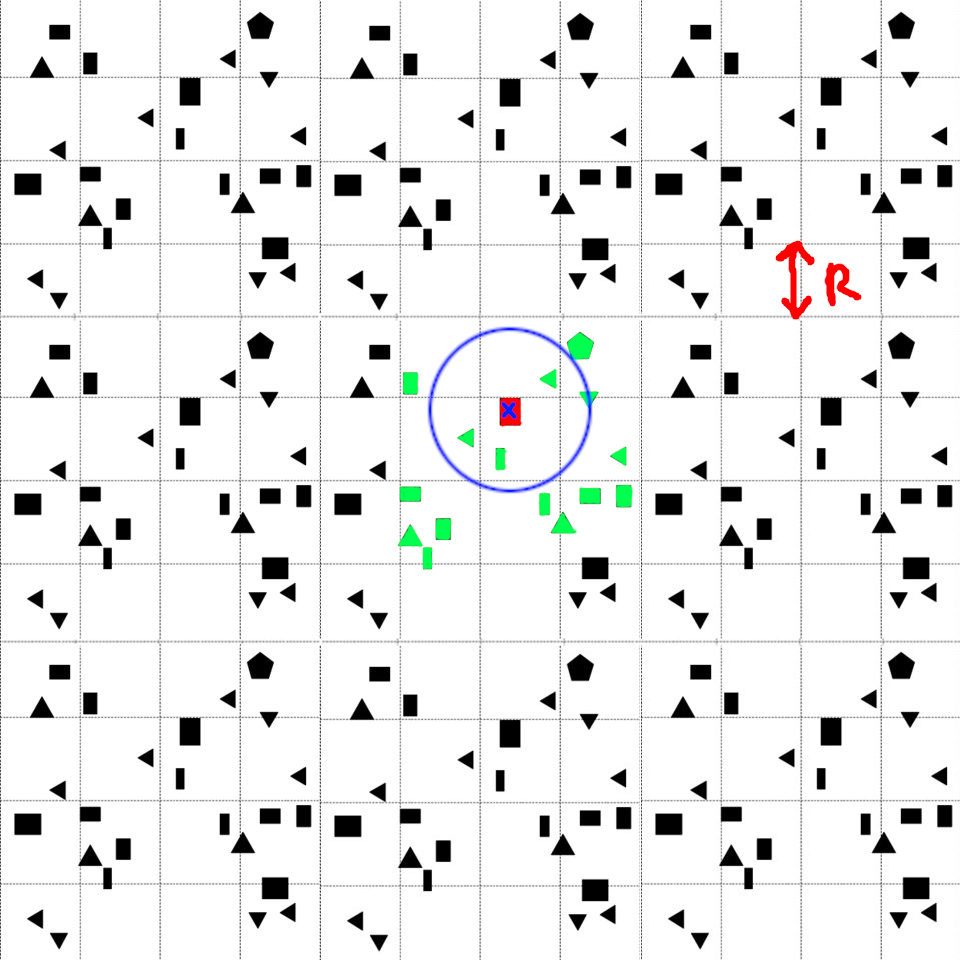
\includegraphics[width=0.4\textwidth]{big_uniform_grid_partitionning}
\end{wrapfigure}
Pour ce faire, nous allons \href{https://en.wikipedia.org/wiki/Space_partitioning}{partitionner l'espace}. C'est à dire que nous allons diviser l'espace et classer les objets de la simulation dans ces divisions selon leur position. Il existe une infinité de façons de diviser l'espace, mais celle que nous allons utiliser est le partitionnement en grille uniforme.

Cette partition est optimale pour un fluide incompressible car au repos il va tendre à une densité homogène dans l'espace de simulation et ainsi il y aura le même nombre de particules dans chacune des divisions.

Si le rayon d'action du noyau est de $R$, on choisit que la longueur du côté du cube de partitionnement soit aussi $R$. Cela permet de n'avoir à prendre en compte que les 8 cellules autour de la cellule où se trouve la particule sur laquelle on travaille.

Par exemple dans le diagramme sur la droite, si on travaille sur la particule en rouge, les seules particules qui ont une chance d'influencer le mouvement de la rouge sont celles en vert.
\\
\\
Dans les faits, pour améliorer les performances nous allons executer l'algorithme suivant à chaque nouvelle image:
\begin{algorithm}
\caption{Table de partition}
\label{CHalgorithm}
\begin{algorithmic}[1]
\Procedure{UpdateSpatialLookup}{}
\For{chaque point $p_i$ de la simulation}
\State (cellX, cellY, cellZ) $\leftarrow$ convertir la position de $p_i$ en les coordonnées de la grille
\State cellKey $\leftarrow$ Hachage(cellX, cellY, cellZ)
\State spatialLookup[$p_i$] $\leftarrow$ ($p_i$, cellKey)
\State startIndices[$p_i$] $\leftarrow +\infty$
\EndFor

\State Trier spatialLookup selon cellKey

\For{chaque point $p_i$ de la simulation}
\State key $\leftarrow$ spatialLookup[$p_i$].cellKey
\If{$p_i=0$}
\State keyPrev $\leftarrow +\infty$
\Else
\State keyPrev $\leftarrow$ spatialLookup[$p_i - 1$].cellKey
\EndIf
\If{key $\neq$ keyPrev}
\State startIndices[key] $\leftarrow$ i
\EndIf
\EndFor

\Return spatialLookup, startIndices
\EndProcedure
\end{algorithmic}
\end{algorithm}

Cet algorithme renvoit deux tables, \textbf{spatialLookup} et \textbf{startIndices}

\end{document}
